\section{Performance Measurement}


\subsection{flips and flops}

\paragraph{flips}  This is intended to measure \emph{instruction} rate through the floating point pipe with no massaging.



\paragraph{flops}  Perhaps the more well-known measurement is the rate of floating point \emph{operations}.  

Calling \code{system.flops(expr)} on a valid \R expression \code{expr} will produce system and processor timings, the number of floating point operations, and the Mflops.

The \code{pca} demo shows off this functionality with principal components analysis.  Executing:
\begin{lstlisting}
demo("pca", "pbdPAPI")
\end{lstlisting}
on an Intel Sandy Bridge Core i5 produces the following outputs:
\begin{Output}
      m  n  measured theoretical difference pct.error   mflops
1 10000 50 211875901   202500000    9375901  4.425185 1637.195
\end{Output}



\paragraph{Theoretical flops}
\begin{align*}
\text{flops} = \text{(\# cores)} * \text{(\# of SSE units per core)} * \text{(cycles / second)} * \text{(\# SSE operations per cycle)}
\end{align*}

single precision (divide by 2 for double precision).

So for this Intel Sandy Bridge Core i5 again as a reference, the 

\begin{align*}
\text{Mflops} &= (4) * (2) * (3200 Mhz) * 2 \\ 
&= 25600 
\end{align*}

or about 25 Gflops (1,000,000,000 flops).




\subsection{Cache Misses and Cache Hits}

\paragraph{Memory and Cache}

Computers operate at \emph{billions} of cycles per second.  Of course, those operations occur on data.  A useful abstraction we use in thinking about processing data is you load the stuff up into ram and then the processor does things to it.  This is usually fine, or at least convenient, but it's not accurate, as you are probably aware.  

\begin{figure}[ht]
  \centering
  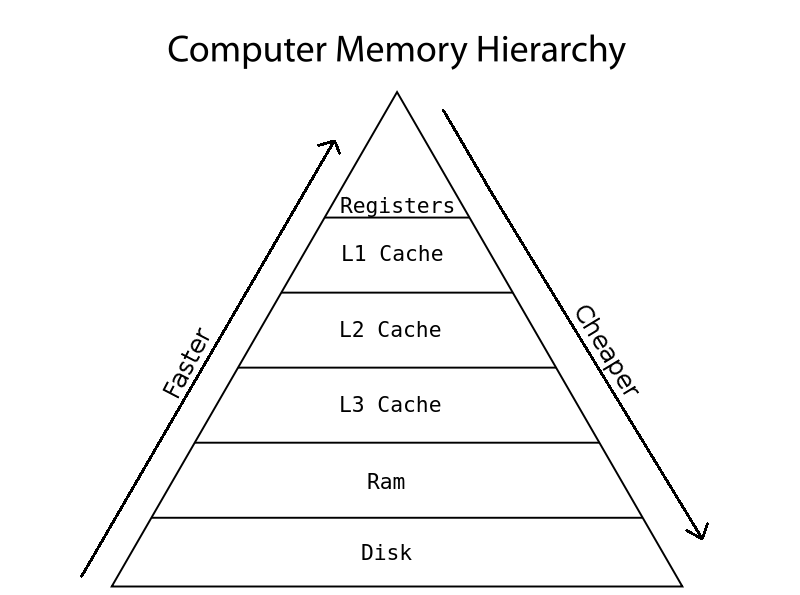
\includegraphics[scale=.54]{./include/pics/memory}
  \caption{Memory Hierarchy}
  \label{fig:mem}
\end{figure}
Another more accurate abstraction is that shown in Figure~\ref{fig:mem}.  In a sense, the magic really happens when things get into the CPU registers.  But something that's in ram that you want to operate on, as it's headed to the CPU, it gets cached into various levels of (comparatively) fast access storage along the way. Not understanding this (simplified from reality) architecture can have can cause some pretty nasty performance side-effects. on your code.
\begin{figure}[ht]
  \centering
  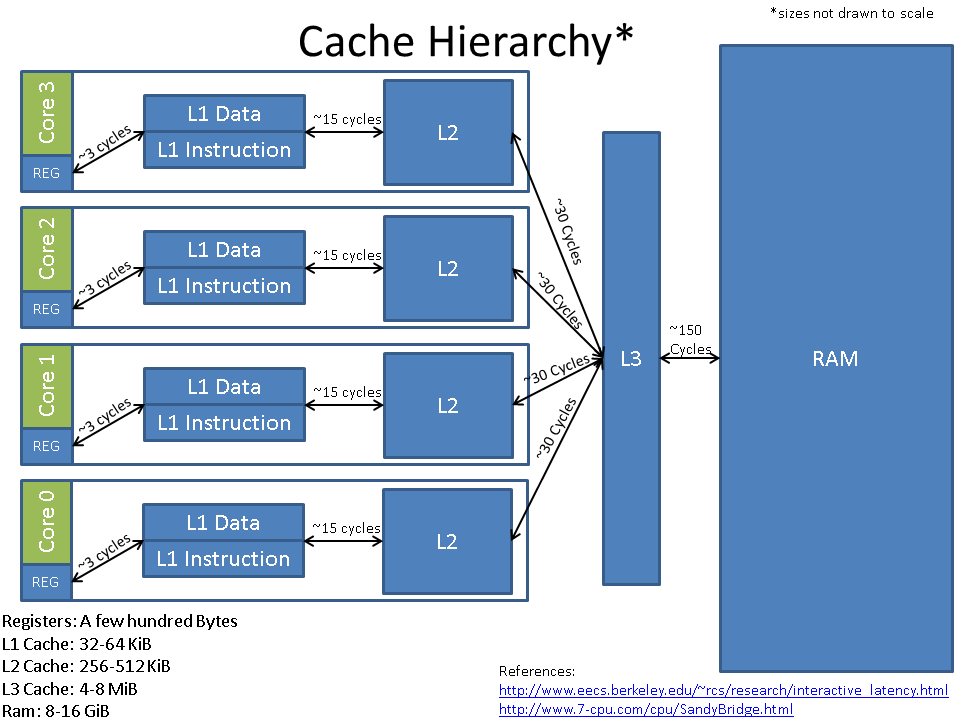
\includegraphics[scale=.5]{./include/pics/cache}
  \caption{Still from Interactive Visualization Showing Relative Memory Access Speeds}
  \label{fig:cache}
\end{figure}
If you're unfamiliar with this, I would strongly encourage you to check out this really cool interactive
\href{http://www.overbyte.com.au/misc/Lesson3/CacheFun.html}{visualization} 
showing (relative) speeds of cache misses, also shown in Figure~\ref{fig:cache}.  It too involves some hefty simplifications of how modern hardware actually works, so if this is at all confusing, let us all take a moment to pity the tragic life of the computer engineer.


\paragraph{Cache Misses} Fundamentally, a cache miss occurs when the cache needs some piece of data to pass along to registers, but it isn't immediately available and has to go digging through ram (or god help you, disk) to get it.  Cache misses are bad and reduce performance.  You can't get rid of them, unless your entire problem fits into cache (which is glorious when it happens), but you can eliminate \emph{unnecessary} cache misses being aware of how your data and algorithms interact with cache.  When people tell you things like ``R's matrices are column-major'' or that you should loop over columns then rows, this is exactly what they are talking about.

Consider the following example, where we will fill a matrix with 1's, first by looping over rows then columns, and then by looping over columns then rows.  For maximum effect, we will be dropping to \C by way of \pkg{Rcpp}.  If you do not have \pkg{Rcpp} installed on your system, you can still follow along (even if you don't know \CXX), but you will not be able to recreate the timings locally.
\begin{lstlisting}
library(inline)

bad_cache_access <- "
  int i, j;
  const int n = INTEGER(n_)[0];
  Rcpp::NumericMatrix x(n, n);
  
  
  for (i=0; i<n; i++)
    for (j=0; j<n; j++)
      x(i, j) = 1.;
  
  return x;
"

good_cache_access <- "
  int i, j;
  const int n = INTEGER(n_)[0];
  Rcpp::NumericMatrix x(n, n);
  
  
  for (j=0; j<n; j++)
    for (i=0; i<n; i++)
      x(i, j) = 1.;
  
  return x;
"


bad <- cxxfunction(signature(n_="integer"), body=bad_cache_access, plugin="Rcpp")
good <- cxxfunction(signature(n_="integer"), body=good_cache_access, plugin="Rcpp")
\end{lstlisting}

A quick check of run times shows something drastically different happening:
\begin{Output}
system.time(bad(n))
#   user  system elapsed 
#  1.016   0.232   1.259 

system.time(good(n))
#   user  system elapsed 
#  0.201   0.155   0.357 
\end{Output}

So even though we (mathematically) are doing the exact same thing, the run times differ by a factor of 3.5.  \thispackage allows us to more thoroughly see what's happening.  If we use \code{papi.cache()} to check the L1, L2, and L3 cache misses for each of these functions:
\begin{Output}
library(pbdPAPI)
n <- 10000L

papi.cache(bad(n))
#$L1.total
#[1] 193580295
#
#$L2.total
#[1] 159442230
#
#$L3.total
#[1] 16895275

papi.cache(good(n))
#$L1.total
#[1] 15552007
#
#$L2.total
#[1] 11580023
#
#$L3.total
#[1] 801150
\end{Output}

it should be readily apparent what is going on now.  The L1 cache misses differ by more than an order of magnitude, 194 million to 16 million!